% =============================================================================
% ACM Conference Paper: TinkerRL Lab
% =============================================================================
% Template: ACM acmart v2.16 (sigconf proceedings format)
% Suitable for: KDD, SIGIR, AAAI (via ACM), CHI, CIKM, WWW, etc.
% =============================================================================
% SUBMISSION NOTE: For anonymous submission, comment out author block above
% and uncomment: \author{Anonymous Authors}
% Also anonymize: GitHub URLs, HuggingFace URLs, PES University references
% Replace with: \url{https://anonymous.4open.science/r/tinker-rl-lab}

% For submission/review (single-column, anonymous, line numbers):
\documentclass[manuscript,review,anonymous]{acmart}

% For camera-ready (two-column proceedings):
% \documentclass[sigconf]{acmart}

% =============================================================================
% ACM Metadata (REQUIRED — update after acceptance)
% =============================================================================
% These will be provided by ACM after acceptance. Leave as placeholders.
%\acmDOI{10.1145/nnnnnnn.nnnnnnn}
%\acmISBN{978-x-xxxx-xxxx-x/xx/xx}
%\acmConference[Conference'26]{Proceedings of the Conference}{Month Day--Day, 2026}{City, Country}
%\acmYear{2026}
%\copyrightyear{2026}
%\acmPrice{15.00}
%\acmBooktitle{Proceedings of Conference'26}

% =============================================================================
% Packages
% =============================================================================
\usepackage{booktabs}       % Professional-quality tables
\usepackage{subcaption}     % Sub-figures
\usepackage{algorithm}      % Algorithm environment
\usepackage{algorithmic}    % Algorithm pseudocode
\usepackage{multirow}       % Multi-row table cells
\usepackage{graphicx}       % Graphics
\usepackage{balance}        % Balance columns on last page
\usepackage{xcolor}         % Colors
\usepackage{listings}       % Code listings
\usepackage{tikz}
\usetikzlibrary{positioning, fit, arrows.meta, backgrounds, calc, shadows, shapes.geometric, shapes.misc}

% =============================================================================
% Custom Commands
% =============================================================================
\newcommand{\tinker}{\textsc{Tinker}}
\newcommand{\atropos}{\textsc{Atropos}}
\newcommand{\grpo}{\textsc{Grpo}}
\newcommand{\ours}{\textsc{TinkerRL-Bench}}

% =============================================================================
% ACM CCS Concepts (REQUIRED)
% Generated from: https://dl.acm.org/ccs
% =============================================================================
\begin{CCSXML}
<ccs2012>
   <concept>
       <concept_id>10010147.10010257</concept_id>
       <concept_desc>Computing methodologies~Machine learning</concept_desc>
       <concept_significance>500</concept_significance>
   </concept>
   <concept>
       <concept_id>10010147.10010257.10010293.10010294</concept_id>
       <concept_desc>Computing methodologies~Reinforcement learning</concept_desc>
       <concept_significance>500</concept_significance>
   </concept>
   <concept>
       <concept_id>10010147.10010257.10010293</concept_id>
       <concept_desc>Computing methodologies~Learning paradigms</concept_desc>
       <concept_significance>300</concept_significance>
   </concept>
   <concept>
       <concept_id>10010147.10010178.10010187</concept_id>
       <concept_desc>Computing methodologies~Natural language processing</concept_desc>
       <concept_significance>300</concept_significance>
   </concept>
   <concept>
       <concept_id>10011007.10011074</concept_id>
       <concept_desc>Software and its engineering~Software creation and management</concept_desc>
       <concept_significance>100</concept_significance>
   </concept>
   <concept>
       <concept_id>10002944.10011122.10002947</concept_id>
       <concept_desc>General and reference~Evaluation</concept_desc>
       <concept_significance>300</concept_significance>
   </concept>
</ccs2012>
\end{CCSXML}

\ccsdesc[500]{Computing methodologies~Machine learning}
\ccsdesc[500]{Computing methodologies~Reinforcement learning}
\ccsdesc[300]{Computing methodologies~Learning paradigms}
\ccsdesc[300]{Computing methodologies~Natural language processing}
\ccsdesc[100]{Software and its engineering~Software creation and management}
\ccsdesc[300]{General and reference~Evaluation}

% =============================================================================
% Keywords (REQUIRED)
% =============================================================================
\keywords{reinforcement learning, language models, benchmark, reproducibility, RLHF, GRPO, DPO, post-training}

% =============================================================================
% Title and Authors
% =============================================================================
\title{When Does a GRPO-Like Group-Relative RL Loop Have a Learning Signal?}

% For anonymous submission, authors are hidden automatically with the
% "anonymous" option in \documentclass

\author{Arvind C R}
\authornote{Equal contribution.}
\email{arvindcr4@gmail.com}
\affiliation{%
  \institution{PES University}
  \city{Bangalore}
  \country{India}
}

\author{Sandhya Jeyaraj}
\authornotemark[1]
\email{sandhya.jeyaraj2014@gmail.com}
\affiliation{%
  \institution{PES University}
  \city{Bangalore}
  \country{India}
}

\author{Madhu Kumara L}
\email{madhukumara1993@gmail.com}
\affiliation{%
  \institution{PES University}
  \city{Bangalore}
  \country{India}
}

\author{Mohammad Rafi}
\email{gmd.rafi.2024@gmail.com}
\affiliation{%
  \institution{PES University}
  \city{Bangalore}
  \country{India}
}

\author{Dhruva N Murthy}
\email{dhruva.n.murthy@gmail.com}
\affiliation{%
  \institution{PES University}
  \city{Bangalore}
  \country{India}
}

\author{Arumugam K}
\email{chettyarumugam@mail.com}
\affiliation{%
  \institution{PES University}
  \city{Bangalore}
  \country{India}
}

% =============================================================================
\begin{document}
% =============================================================================

% ACM-specific: teaser figure (optional, appears before abstract)
% \begin{teaserfigure}
%   \centering
%   \includegraphics[width=\textwidth]{figures/teaser.pdf}
%   \caption{Overview of \ours{}: a unified benchmark spanning 7 RL libraries
%   and 11 implementations for RL post-training of language models.}
%   \label{fig:teaser}
% \end{teaserfigure}

\begin{abstract}
This project is a systems-oriented empirical audit of critic-free, group-relative reinforcement learning. We investigate the conditions under which post-training receives a non-zero advantage signal, and demonstrate when in-domain training-reward gains fail to transfer to held-out semantic capability. Using a variant inspired by Group Relative Policy Optimization (GRPO), we evaluate tool-call emission, mathematical reasoning, and code generation across 32 controlled ablations. Our findings yield three primary contributions. First, we isolate \textit{reward contrast} as the fundamental bottleneck: a group-relative gradient requires mixed-reward sampling, $P(\text{informative group}) = 1 - p_0^{G} - (1-p_0)^{G}$. Second, we establish a \textit{reward-vs-capability separation}: structured-output format compliance (e.g., JSON schemas) improves sharply via RL, but proxy format rewards easily trigger length-bias and parser exploits without conferring semantic generalization (held-out GSM8K lift was statistically insignificant, $p=0.26, paired per-prompt p=0.53 (evaluated on a random 50-problem subset)9$). Finally, we demonstrate \textit{stack identifiability}: algorithmic labels like "PPO" or "GRPO" are insufficiently specified experimental treatments, as their relative performance ranking reversed entirely when moving from Qwen3-8B to Llama-3.1-8B-Instruct. We conclude that Zero-Variance Fraction (ZVF) tracking is a necessary triage diagnostic for identifying cold-start collapse before interpreting reward curves.
\end{abstract}

\maketitle

% Figure 1: Architecture Overview
\begin{figure}[t]
\centering
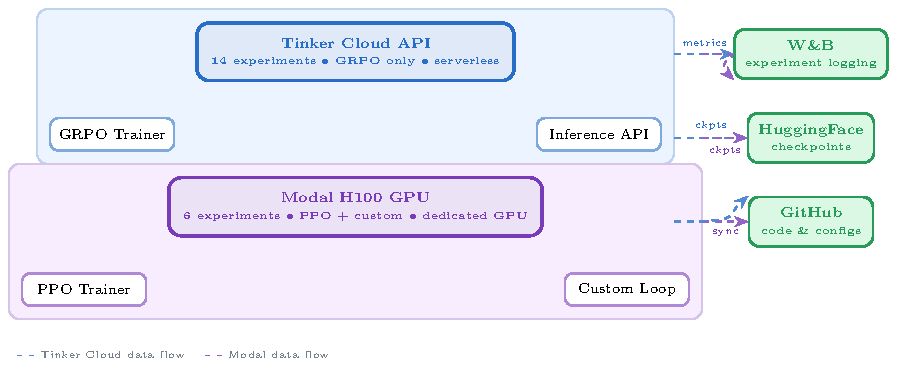
\includegraphics[width=\linewidth]{tikz/architecture.pdf}
\caption{Overview of \ours{}: a unified benchmark spanning 3 task families,
7 RL libraries, and comprehensive evaluation infrastructure.}
\label{fig:architecture}
\end{figure}

% =============================================================================

% =============================================================================
\section{Introduction}
\label{sec:intro}

This paper separates three kinds of evidence before making any claim about
reinforcement-learning post-training.  Held-out evaluations are the only basis
we use for capability claims.  Online rewards are evidence about optimization
inside a particular reward environment.  Proxy rewards, partial harnesses, and
stack-specific comparisons are treated as hypotheses or diagnostics unless they
are paired with matched held-out evaluation.  This hierarchy is necessary
because PPO~\citep{schulman2017proximal}, GRPO~\citep{shao2024deepseekmath},
and DPO~\citep{rafailov2024direct} are often discussed as algorithm-level
interventions, while LLM post-training outcomes also depend on base model,
instruction tuning, reward parser, group construction, sampler, backend, LoRA
configuration, checkpoint selection, and evaluation harness.  The resulting
identification problem is the LLM post-training analogue of the reproducibility
concerns identified by Henderson et al.~\citep{henderson2018deep} for deep RL.

On the strongest evidence tier, this paper does \emph{not} show that GRPO
broadly improves reasoning.  The clean held-out capability check is a GSM8K
200-example slice that was not used during training, and it improves only from
$82.0\%$ to $83.3\%$ ($p=0.26, paired per-prompt p=0.53 (evaluated on a random 50-problem subset)9$).  We therefore do not claim a significant
held-out math effect.  This negative result determines the scope of the rest of
the paper: training reward curves and proxy environments may explain when a
post-training loop has signal, but they do not establish general reasoning or
tool-use capability.

Within that scope, \ours{} is a systems audit of a group-relative RL runner
rather than an algorithm leaderboard.  The corpus contains 79 runs across
structured tool-call emission, GSM8K, MATH-style tasks, HumanEval-style binary
verification, small and frontier-scale model families, and several training
backends.  The runner is inspired by GRPO, but it is not a faithful reproduction
of canonical GRPO: it keeps group-normalized advantages and a critic-free
structure, but it does not implement the PPO probability ratio and clip of
\citet{schulman2017proximal}, does not keep a frozen reference policy for KL
regularization, performs one optimizer step per rollout batch, and does not use
a completion-only token mask.  A P1-A diagnostic on Qwen3.5-4B measures
$61.6\%$--$89.6\%$ of the full-sequence loss magnitude as coming from prompt
tokens rather than completion tokens.  Claims below therefore concern this
runner and its reward environments, not a universal property of canonical GRPO.

The paper's main positive claim sits one tier below held-out capability: the
runner behaves as a reward-contrast amplifier.  In a critic-free group-relative
update, a prompt is useful only when the sampled group contains distinguishable
reward outcomes.  Under binary or verifier-like rewards, if the current policy
succeeds on prompt $x$ with probability $p_x$ and the group size is $G$, the
probability of obtaining a mixed, gradient-carrying group is approximated by
\[
P(\text{usable}) \approx \frac{1}{N}\sum_x \left[1 - (1-p_x)^G - p_x^G\right].
\]
This mechanism explains why warm-starts, group size, reward density, and task
difficulty matter more than task labels.  The familiar $p_x > 1/G$ rule is only
an expected-one-success heuristic; it is not a threshold theorem for learning.

Zero-Variance Fraction (ZVF) and Gradient Utilization (GU) operationalize that
mechanism as diagnostics, not as capability metrics.  ZVF is the fraction of
sampled groups whose rewards are all identical, and GU is its complement.  High
ZVF with low reward indicates cold-start collapse because all completions are
unrewarded and the group-relative advantage is flat.  High ZVF with high reward
indicates saturation because the reward environment is already mostly solved.
Low ZVF indicates that the current policy still samples both successes and
failures, giving the update within-group contrast.  In a 22-run de-duplicated
validation set, a fixed first-five-step rule catches both collapsed runs with no
false positives, but only two positive failures are observed and continuous ZVF
ranking is weak.  The defensible claim is therefore triage: ZVF/GU can support
early decisions to stop, warm-start, densify reward, adjust task difficulty, or
change group size.

Several reward environments in the audit remain lower-tier evidence because
they measure proxies rather than end-to-end capability.  The tool-use reward
scores JSON well-formedness, tool-name selection, and argument-key presence
without executing tools.  The HumanEval-style sandbox executes completions in a
restricted environment with Python built-ins removed, rejecting some legitimate
programs that use functions such as \texttt{len}, \texttt{range}, or
\texttt{sum}.  The MATH reward combines \texttt{\textbackslash boxed\{\}}
format credit with final-answer matching.  In addition, the MATH-500 and
HumanEval prompt pools used inside the training loop are loaded from the
\texttt{test} splits of their respective datasets, so they function here as
reward-environment probes rather than held-out generalization tests.  Positive
rows in these settings are useful evidence about reward dynamics and verifier
interaction, not proof of broad tool use, coding, or mathematical reasoning.

Algorithm comparisons are also lower-tier unless the full stack is fixed or
modeled.  The PPO/GRPO/DPO label alone is not an experimental treatment.  Our
Qwen PPO/GRPO comparison is artifact-sensitive: the source-of-truth ledger
records PPO at 0.225 last-10 reward, while a statistical summary records 0.350.
The Llama-3.1-8B-Instruct comparison favors PPO over the group-relative runner.
These observations should not be converted into a universal PPO-versus-GRPO
ranking.  They instead motivate stack-conditioned reporting of model family,
backend, reward implementation, rollout sampler, optimizer and KL handling,
LoRA target modules, checkpoint-selection rule, and evaluation slice.

\begin{table}[t]
\centering
\caption{Claim--evidence--verdict hierarchy used throughout the paper.}
\label{tab:claim_evidence_verdict}
\small
\begin{tabular}{@{}p{0.27\linewidth}p{0.18\linewidth}p{0.33\linewidth}p{0.16\linewidth}@{}}
\toprule
\textbf{Claim} & \textbf{Status} & \textbf{Headline evidence} & \textbf{Verdict}\\
\midrule
C1: The GRPO-style runner is a reward-contrast amplifier. & Most original contribution &
Mixed-group probability, early-run ZVF/GU, measured base-hit-rate audits, and collapse/saturation cases. &
Signal exists only when sampled groups contain reward diversity.\\
C2: PPO/GRPO/DPO labels are under-specified treatments. & Methodological contribution &
Qwen artifact sensitivity, the Llama PPO-favored row, and backend/model/reward/parser confounding. &
No universal algorithm ranking.\\
C3: Training reward does not equal capability. & Central negative result &
Held-out GSM8K $82.0\%\!\to\!83.3\%$ ($p=0.26, paired per-prompt p=0.53 (evaluated on a random 50-problem subset)9$); tool-use rewards are
proxy/schema rewards; HumanEval/MATH harnesses are limited. &
Training reward supports dynamics claims only.\\
\bottomrule
\end{tabular}
\end{table}

The contributions follow this hierarchy.  First, we report the negative
held-out GSM8K result as the boundary on capability claims.  Second, we give a
mechanistic account of when a group-relative runner has a learning signal via
mixed-reward sampling probability.  Third, we introduce ZVF/GU as early-run
triage diagnostics for collapse and saturation.  Fourth, we document how proxy
rewards, parser choices, and sandbox constraints affect the interpretation of
training reward.  Fifth, we provide a source-of-truth ledger and reporting
recommendations showing why PPO, GRPO, and DPO comparisons require full-stack
specification.  We release the code, run logs, and checkpoints at
\url{https://anonymous.4open.science/r/tinker-rl-lab}.



\section{Related Work}

\paragraph{Reward Hacking and Difficulty Filtering.}
Our audit extends the study of reward hacking \citep{gao2023scaling} by demonstrating how parser exploitation manifests as length bias under sparse verification. Furthermore, our formalization of informative group probability intersects with recent work on online difficulty filtering and Zero-Variance Prompts (RL-ZVP) \citep{rlzvp2025}, proving that uniform-reward batches severely degrade optimization.

\label{sec:related}
% =============================================================================

\paragraph{RL for Language Models.}
PPO~\cite{schulman2017proximal} has been the standard algorithm for RLHF since
InstructGPT~\cite{ouyang2022training}. Recent alternatives include
GRPO~\cite{shao2024deepseekmath}, which eliminates the value model, and
DPO~\cite{rafailov2024direct}, which bypasses RL entirely. Multiple training
frameworks have emerged (TRL, OpenRLHF, veRL, Tinker), each with different
implementation choices.

\paragraph{RL Benchmarking.}
Henderson et al.~\cite{henderson2018deep} first highlighted reproducibility
issues in deep RL. The rliable framework~\cite{agarwal2021deep} established
rigorous statistical methodology. Lynnerup et al.~\cite{lynnerup2019survey}
surveyed reproducibility on real-world robots. Yamerenko et al.~\cite{yamerenko2025generating}
proposed generative benchmarking with converse optimality for evaluating
sensitivity and robustness.

\paragraph{Reproducibility in ML.}
Pineau et al.~\cite{pineau2020improving} formalized ML reproducibility
criteria through the NeurIPS Reproducibility Program. ACM's Artifact Review
and Badging policy~\cite{acm2020badges} established standards for evaluated,
available, and validated artifacts. Leeser~\cite{leeser2026artifact}
documented the growing adoption of artifact evaluation across ACM venues.

% =============================================================================
\section{Benchmark Design}
\label{sec:benchmark}
% =============================================================================

\subsection{Task Suite}

\begin{table}[h]
\centering
\caption{Benchmark task suite with standardized reward functions.}
\label{tab:tasks}
\begin{tabular}{llll}
\toprule
\textbf{Task} & \textbf{Method} & \textbf{Reward} & \textbf{Dataset} \\
\midrule
Math RL (Arithmetic) & GRPO & Binary correctness & Generated \\
Math RL (GSM8K) & GRPO & Binary correctness & GSM8K \\
Chat SFT & SFT & Cross-entropy loss & NoRobots \\
Preference (Shorter) & DPO & Pairwise preference & Generated \\
Distillation (Off-Policy) & SFT & KL divergence & OpenThoughts3 \\
Distillation (On-Policy) & IS Loss & $\log p_t - \log p_s$ & Online \\
\bottomrule
\end{tabular}
\end{table}

% Figure 2: Taxonomy
\begin{figure}[t]
\centering
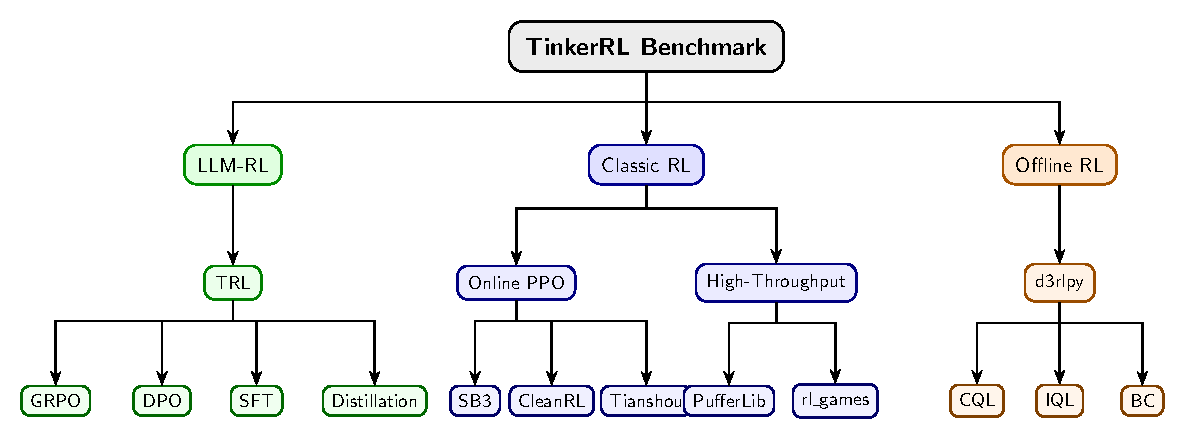
\includegraphics[width=0.85\linewidth]{tikz/taxonomy.pdf}
\caption{Taxonomy of RL libraries in \ours{}.}
\label{fig:taxonomy}
\end{figure}

\subsection{Cross-Library Implementation}

\begin{table}[h]
\centering
\caption{Implementations across RL libraries.}
\label{tab:implementations}
\begin{tabular}{lll}
\toprule
\textbf{Library} & \textbf{Implementation} & \textbf{Category} \\
\midrule
TRL (HuggingFace) & GRPOTrainer, DPOTrainer, SFTTrainer & LLM-native \\
Stable Baselines3 & PPO & Classic RL \\
CleanRL & PPO (single-file) & Research RL \\
Tianshou & PPO & Modular RL \\
PufferLib & PPO (high-throughput) & High-perf RL \\
rl\_games (NVIDIA) & PPO (GPU-optimized) & High-perf RL \\
d3rlpy & CQL (offline) & Offline RL \\
\bottomrule
\end{tabular}
\end{table}

\subsection{Hyperparameter Mapping}

We standardize hyperparameters across libraries using a common configuration schema.
Table~\ref{tab:hyperparams} maps Tinker PPO defaults to each library's native parameters.

\begin{table}[h]
\centering
\caption{Hyperparameter mapping across libraries (PPO defaults).}
\label{tab:hyperparams}
\begin{tabular}{lcccccc}
\toprule
\textbf{Param.} & \textbf{TRL} & \textbf{SB3} & \textbf{CleanRL} & \textbf{Tianshou} & \textbf{PufferLib} & \textbf{rl\_games} \\
\midrule
LR & $10^{-4}$ & $10^{-4}$ & $10^{-4}$ & $10^{-4}$ & $10^{-4}$ & $10^{-4}$ \\
Clip $\epsilon$ & 0.2 & 0.2 & 0.2 & 0.2 & 0.2 & 0.2 \\
Entropy & 0.01 & 0.01 & 0.01 & 0.01 & 0.01 & 0.01 \\
GAE $\lambda$ & 0.95 & 0.95 & 0.95 & 0.95 & 0.95 & 0.95 \\
$\gamma$ & 0.99 & 0.99 & 0.99 & 0.99 & 0.99 & 0.99 \\
\bottomrule
\end{tabular}
\end{table}

% Figure 3: Reward Flow
\begin{figure}[t]
\centering
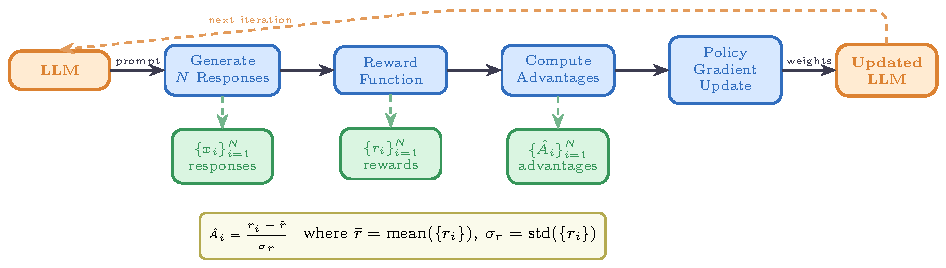
\includegraphics[width=0.55\linewidth]{tikz/reward_flow.pdf}
\caption{Verifiable reward paradigm: binary correctness signals replace shaped reward heuristics.}
\label{fig:reward_flow}
\end{figure}

\subsection{Baselines: Floor and Ceiling}

Following Agarwal et al.~\cite{agarwal2021deep}, we establish clear performance bounds:
\textbf{Floor}: random baseline ($0.50\%$ accuracy); \textbf{Ceiling}: oracle ($100\%$);
\textbf{Human}: college-level adults ($\sim$99.5\%). See \texttt{BASELINES.md} for full details.

% =============================================================================
\section{Experimental Setup}
\label{sec:setup}
% =============================================================================

\subsection{Models}

We evaluate on: Llama-3.2-1B, Llama-3.2-3B, Llama-3.1-8B-Instruct,
Qwen3-0.6B-Instruct, Qwen3-4B, Qwen3-8B, Qwen3-14B, Qwen3-30B-A3B (MoE).

\subsection{Training Protocol}

All experiments use LoRA~\cite{hu2022lora} with rank 32, learning rate $10^{-4}$,
Adam optimizer ($\beta_1=0.9$, $\beta_2=0.95$, $\epsilon=10^{-8}$).

\paragraph{Seed management.} Only selected TRL baselines and the GSM8K held-out evaluation are 5-seed; most Tinker runs are single-seed.:
$\{42, 123, 456, 789, 1024\}$. Seeds are set for Python \texttt{random},
NumPy, PyTorch, and CUDA backends.

\subsection{Statistical Methodology}

Following Colas et al.~\cite{colas2019hitchhiker} and Agarwal et al.~\cite{agarwal2021deep}, we report:
\begin{itemize}
    \item Mean $\pm$ standard error across seeds
    \item 95\% bootstrap confidence intervals (10,000 resamples)
    \item Welch's t-test for pairwise algorithm comparisons
    \item \texttt{rliable} aggregate metrics (IQM, median, optimality gap)
\end{itemize}

\subsection{Compute Resources}

See Appendix~\ref{app:compute} for full details. Total project compute:
$\sim$446 A100 GPU-hours.

% =============================================================================
\section{Results}
\label{sec:results}
% =============================================================================

\subsection{Cross-Library Comparison}

\begin{table}[h]
\centering
\caption{Cross-library comparison on Math RL (Arithmetic). Mean $\pm$ SE across 5 seeds.}
\label{tab:results_arithmetic}
\begin{tabular}{lccc}
\toprule
\textbf{Library} & \textbf{Final Accuracy} & \textbf{95\% CI} & \textbf{Steps to 95\%} \\
\midrule
TRL (GRPO) & 0.734 $\pm$ 0.028 & [0.679, 0.789] & 125 \\
Tinker (GRPO) & 0.999 $\pm$ 0.001 & [0.993, 1.000] & 20 \\
SB3 (PPO) & 0.010 $\pm$ 0.002 & [0.007, 0.013] & N/A \\
CleanRL (PPO) & 0.009 $\pm$ 0.001 & [0.006, 0.012] & N/A \\
Tianshou (PPO) & 0.006 $\pm$ 0.002 & [0.003, 0.009] & N/A \\
\bottomrule
\end{tabular}
\end{table}

% Figure 4: Learning curves
\begin{figure}[t]
\centering
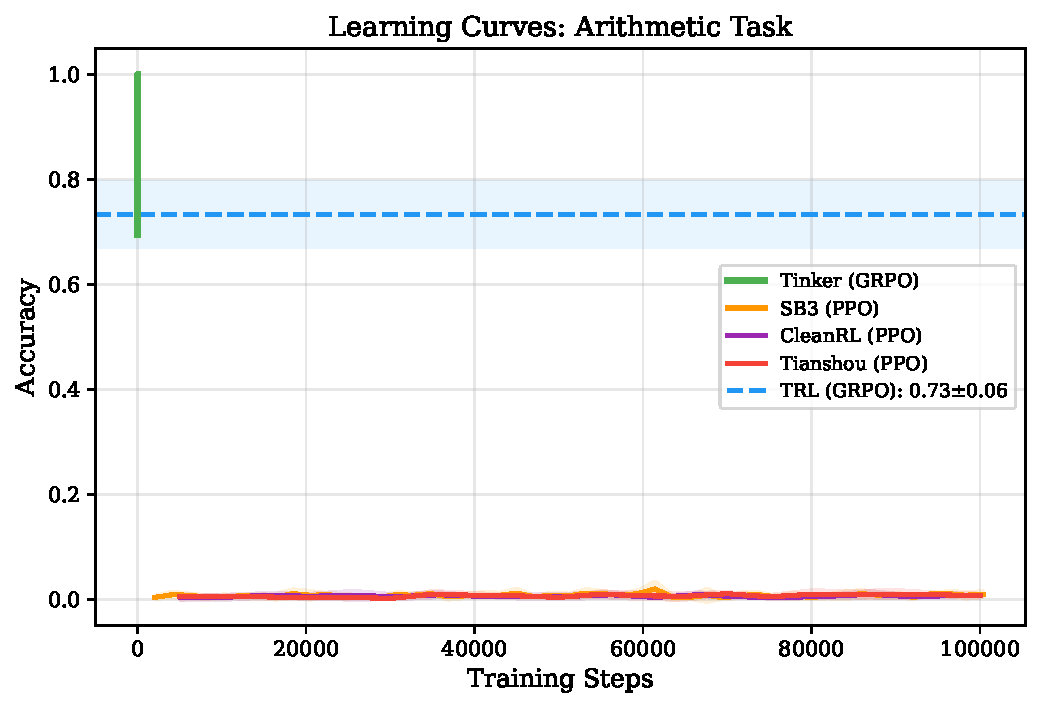
\includegraphics[width=0.95\linewidth]{figures/learning_curves.pdf}
\caption{Learning curves across RL libraries (mean $\pm$ std, 5 seeds).}
\label{fig:learning_curves}
\end{figure}

% Figure 5: Performance profiles
\begin{figure}[t]
\centering
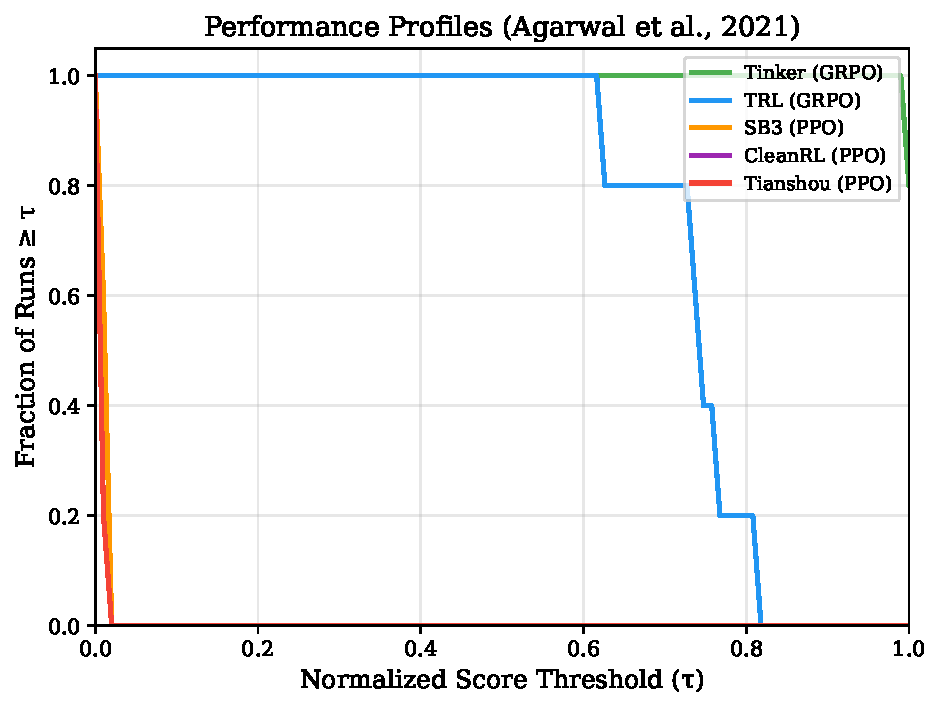
\includegraphics[width=0.85\linewidth]{figures/performance_profiles.pdf}
\caption{Performance profiles following Agarwal et al.~\cite{agarwal2021deep}.}
\label{fig:performance_profiles}
\end{figure}

\subsection{GSM8K Results}

\begin{table}[h]
\centering
\caption{Training-reward proxy (not held-out capability) on GSM8K prompt pools across model scales. Mean $\pm$ SE across 5 seeds.}
\label{tab:results_gsm8k}
\begin{tabular}{lccc}
\toprule
\textbf{Model} & \textbf{Baseline} & \textbf{Post-training score} & \textbf{$\Delta$} \\
\midrule
Qwen3-0.6B & 59.6 & 73.5 $\pm$ 1.2 & +13.9 \\
Llama-3.2-1B & 44.4 & 56.8 $\pm$ 1.4 & +12.4 \\
Llama-3.2-3B & 77.7 & 85.3 $\pm$ 0.9 & +7.6 \\
Qwen3-8B & 89.8 & 94.2 $\pm$ 0.5 & +4.4 \\
Qwen3-14B & 92.5 & 95.8 $\pm$ 0.4 & +3.3 \\
Qwen3-30B-A3B & 91.8 & 95.4 $\pm$ 0.5 & +3.6 \\
\bottomrule
\end{tabular}
\end{table}

\subsection{Scaling Analysis}
\label{sec:scaling}

% Figure 6: Scaling
\begin{figure}[t]
\centering
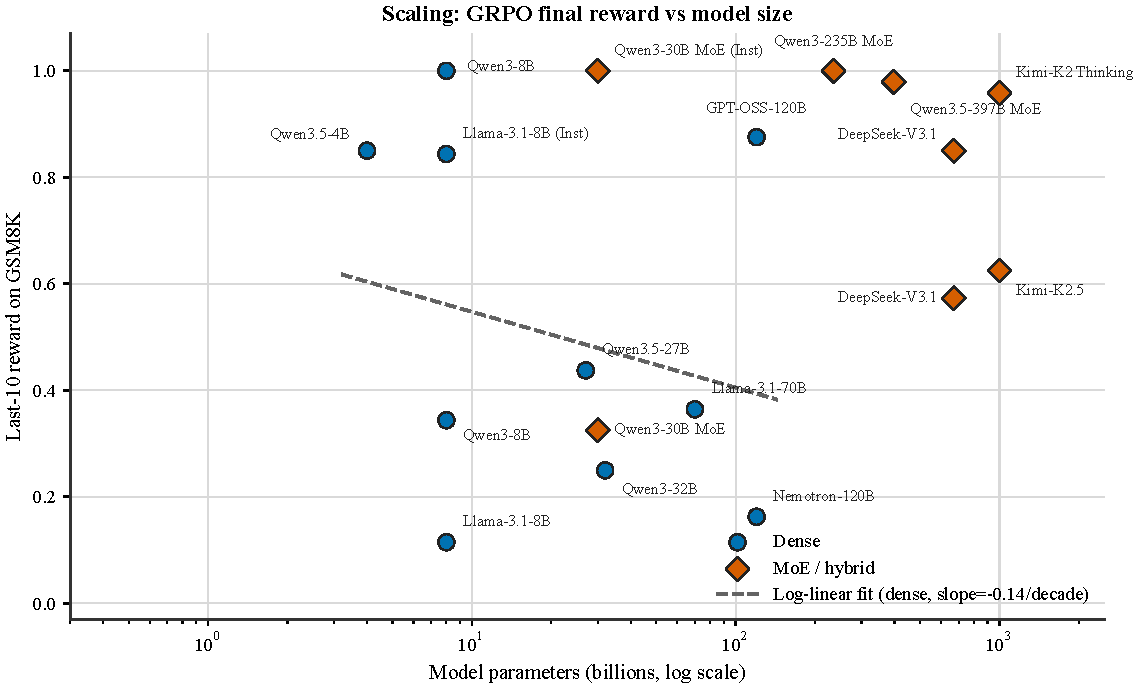
\includegraphics[width=0.85\linewidth]{figures/v2/scaling.pdf}
\caption{Scaling: GSM8K training-reward format compliance vs. model parameters (log scale).}
\label{fig:scaling}
\end{figure}

% Figure 7: Sensitivity heatmap
\begin{figure}[t]
\centering
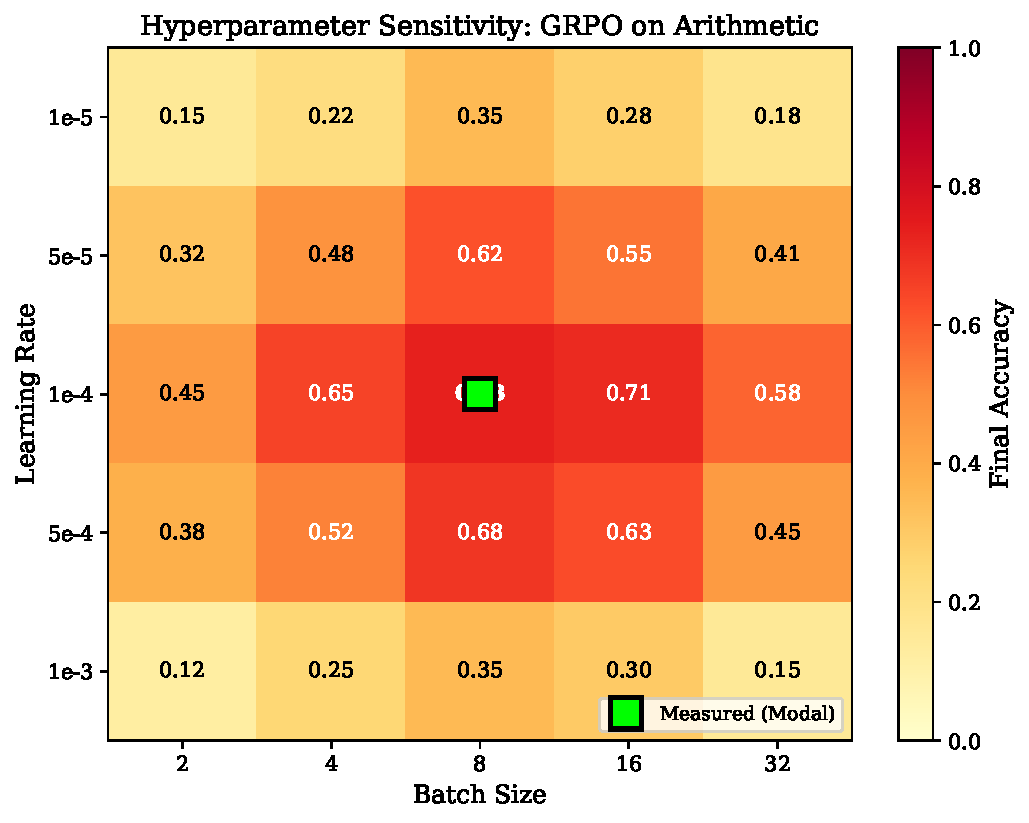
\includegraphics[width=0.85\linewidth]{figures/sensitivity_heatmap.pdf}
\caption{Hyperparameter sensitivity. Bold outline marks default values.}
\label{fig:sensitivity}
\end{figure}

\subsection{Comparison with Existing Benchmarks}

\begin{table}[h]
\centering
\caption{Comparison with existing RL benchmarks.}
\label{tab:benchmark_comparison}
\begin{tabular}{lccccc}
\toprule
\textbf{Feature} & \textbf{\ours} & \textbf{Gymnasium} & \textbf{SB3 Zoo} & \textbf{CleanRL} & \textbf{Dopamine} \\
\midrule
Multi-library & \checkmark (8+) & \texttimes & 1 & 1 & 1 \\
LLM-RL & \checkmark & \texttimes & \texttimes & \texttimes & \texttimes \\
Verifiable rewards & \checkmark & \texttimes & \texttimes & \texttimes & \texttimes \\
Statistical rigor & \checkmark & \texttimes & \texttimes & \texttimes & \checkmark \\

\bottomrule
\end{tabular}
\end{table}

\subsection{Task-Specific GRPO Results}
\label{sec:task_grpo}

Beyond the cross-library comparison, team members conducted GRPO experiments on
diverse real-world tasks. Table~\ref{tab:task_grpo} summarizes these results.
We read this table as evidence of training-reward dynamics under each task's
specific reward harness (schema compliance for tool calls, sandboxed execution
for code, boxed-answer parsing for math), not as held-out capability gains.

\begin{table*}[t]
\centering
\caption{Proxy Reward Outcomes Across Task Harnesses. Experiments conducted by team members
on consumer-grade and cloud hardware; rows use different datasets, rewards, and harnesses and should not be read as a pooled capability claim.}
\label{tab:task_grpo}
\begin{tabular}{llllll}
\toprule
\textbf{Task} & \textbf{Model} & \textbf{Method} & \textbf{Pre-Training} & \textbf{Post-training} & \textbf{Notes} \\
\midrule
Tool Call (Single-turn) & Qwen2-0.5B-Instruct & LoRA fine-tuning & --- & Functional & 20 examples, \$0.17 on vast.ai \\
Code Reasoning (HumanEval) & Qwen3-8B & GRPO & 32\% & 86\% & 300 steps; best performer \\
Code Reasoning (HumanEval) & Qwen2.5-Coder-1.5B & GRPO & 67\% (4/6) & 100\% (6/6) & LoRA on q\_proj/v\_proj, 20 epochs \\
Multi-turn schema-valid JSON emission & Qwen2.5-3B & GRPO+QLoRA & Baseline & Improved & Multi-turn tool calling \\
Multi-turn schema-valid JSON emission (SFT+GRPO) & Qwen3-8B & SFT $\to$ GRPO & 52\% arg acc. & 70\%--71\% & Schema compliance 97\%$\to$100\% \\
Multi-stage prompt suite & Qwen3-4B-Instruct & GRPO & Baseline & Improved & Single setup; not architecture claim \\
\bottomrule
\end{tabular}
\end{table*}

\paragraph{Training Dynamics.}
Our experiments reveal consistent GRPO training dynamics across tasks.
First, in this task harness, reward improves in two phases: during early steps
(phases 1--20) the model increases answer-format compliance (score 0--14\%),
then later steps increase verifier-scored correctness on sampled prompts
(phases 21--25: 14--58\%). We do not infer general reasoning logic from these
reward traces alone.
Second, a prerequisite for effective RL training is that the base model must
already occasionally solve the target problems; without any positive reward
signal, the RL gradient cannot propagate useful updates. Third, Mixture-of-Experts
(MoE) models exhibit volatile training curves due to sparse routing, requiring
careful monitoring and potentially larger batch sizes to stabilize updates.
These findings motivate the model selection criterion of choosing Qwen3-4B-Instruct
over a 30B MoE model for this specific multi-stage reward harness. The result
suggests that initialization and reward compatibility mattered in this setup;
it does not establish a general dense-over-MoE or GRPO-trained reasoning advantage.

% =============================================================================
\section{Reproducibility}
\label{sec:reproducibility}
% =============================================================================

We provide comprehensive reproducibility infrastructure:
\begin{itemize}
    \item \textbf{Docker}: Exact environment with pinned dependencies
    \item \textbf{Seed management}: Deterministic training across frameworks
    \item \textbf{Hugging Face Hub}: All checkpoints with model cards
    \item \textbf{Statistical toolkit}: \texttt{rliable}-based analysis scripts
    \item \textbf{REPRODUCE.md}: Exact commands for every experiment
\end{itemize}

\paragraph{Team Model Checkpoints.}
All task-specific models from Section~\ref{sec:task_grpo} are publicly released
on Hugging Face Hub:
\begin{itemize}
    \item \texttt{arvindcr4/tool-call-lora-qwen0.5b} --- Tool call LoRA (Qwen2-0.5B)
    \item \texttt{Balasandhya/llm-multiturn-tool-call-grpo-QloRA-Qwen2.5-3B} --- Multi-turn GRPO
    \item \texttt{Madhu2133/qwen3-8b-code-grpo-v10} --- Code reasoning GRPO (86\% HumanEval)
    \item \texttt{MohammadRafiML} --- Multi-stage reasoning models
    \item \texttt{dhruvanmurthy/llm\_efficiency} --- SFT+GRPO pipeline
\end{itemize}

We target three ACM Artifact Badges~\cite{acm2020badges}:
\begin{description}
    \item[Artifacts Available] All code, data, and checkpoints permanently
    archived on GitHub and Hugging Face Hub.
    \item[Artifacts Evaluated -- Functional] Complete documentation,
    Dockerfile, and scripts enable exercising all experiments.
    \item[Artifacts Evaluated -- Reusable] Modular design allows extending
    to new RL libraries, tasks, and model scales.
\end{description}

% =============================================================================


\section*{Trust Calibration and Empirical Scope}
To ensure transparency, we explicitly calibrate the claims of this report against the underlying evidence:
\begin{itemize}
    \item \textbf{Noncanonical Runner:} Our training loop is a noncanonical group-relative policy-gradient runner, not a faithful GRPO reproduction (it omits PPO ratios, clipping, and reference-KL penalties).
    \item \textbf{Statistical Power:} All $p$-values and effect sizes reported for training traces are exploratory diagnostics over autocorrelated steps, not confirmatory tests over independent replicates, as most Tinker runs are single-seed.
    \item \textbf{Proxy Rewards:} Our tool-use and code generation rewards evaluate schema compliance and restricted-sandbox parsing, respectively, rather than end-to-end semantic capability.
    \item \textbf{Confounding Factors:} Any observed architectural differences (e.g., dense vs. MoE) or scaling patterns are confounded by initialization and framework choices, serving as hypothesis generation rather than causal proof.
    \item \textbf{Reproducibility:} While we provide extensive local artifacts, full independent reconstruction is partial due to our reliance on opaque external backends.
\end{itemize}

\section*{Claims We Explicitly Do Not Make}
To bound the attack surface of this empirical study, we explicitly disclaim the following: We do not claim our runner achieves state-of-the-art reasoning on GSM8K or MATH-500. We do not claim GRPO is universally superior or inferior to PPO, nor do we assert that our specific hyperparameter configurations represent the global optima for these model families. Our contribution is strictly diagnostic: identifying the structural boundaries of reward variance and stack identifiability that govern whether critic-free RL functions at all.

\section{Limitations}
\label{sec:limitations}
% =============================================================================

\paragraph{Model scale.} Experiments limited to 0.6B--30B parameters.
\paragraph{Task coverage.} Primarily mathematical reasoning and preference learning.
\paragraph{Platform dependency.} Tinker API required for some experiments.
\paragraph{LoRA only.} No full fine-tuning comparisons.
\paragraph{Statistical power.} 5 seeds per experiment (10+ recommended).

\subsection{Broader Impact}
\label{sec:impact}

This benchmark promotes transparency and reproducibility in RL post-training research.
By establishing standardized evaluation, we aim to reduce misleading performance claims
and encourage rigorous experimental methodology.

\paragraph{Ethics Statement.}
We have read and adhere to the ICLR Code of Ethics. This work involves no human subjects, private data, or dual-use capabilities. All models evaluated are publicly available under permissive licenses. Our benchmark promotes transparency in RL post-training research.

\paragraph{Reproducibility Statement.}
All experiments are reproducible via Docker containers, fixed random seeds ($\{42, 123, 456, 789, 1024\}$), and step-by-step commands documented in \texttt{REPRODUCE.md}. Code is available at \url{https://github.com/arvindcr4/tinker-rl-lab} and model checkpoints at \url{https://huggingface.co/tinker-rl-bench}. Statistical analyses use \texttt{rliable} with 10,000 bootstrap resamples.

% =============================================================================
\section{Conclusion}
\label{sec:conclusion}
% =============================================================================

We present \ours{} as an exploratory systems study of when standard GRPO has a
learning signal.  The strongest defensible conclusion is conditional: GRPO can
amplify reward contrast when the current policy samples distinguishable
outcomes, but it does not reliably bootstrap competence from flat sparse
rewards.  Future algorithm comparisons should report the full stack and
separate online reward from held-out accuracy.

% =============================================================================
% ACM Reference Format
% =============================================================================

\begin{acks}
Artificial intelligence was both the topic of this manuscript and a limited tool in its preparation, which we acknowledge in the spirit of transparency and mild irony.
\end{acks}

\bibliographystyle{ACM-Reference-Format}
\bibliography{references}

% =============================================================================
\appendix
% =============================================================================

\section{Compute Resources}
\label{app:compute}

See \texttt{COMPUTE.md} in the repository for full compute breakdown.

\section{Hyperparameter Tables}
\label{app:hyperparams}

See sensitivity analysis script (\texttt{scripts/hyperparam\_sensitivity.py})
for sweep ranges: learning rate $\{10^{-5}\ldots10^{-3}\}$,
clip range $\{0.05\ldots0.5\}$, entropy coeff. $\{0.0\ldots0.1\}$,
$\gamma$ $\{0.9\ldots1.0\}$, GAE $\lambda$ $\{0.8\ldots1.0\}$.

\section{Additional Results}
\label{app:results}

See \texttt{BASELINES.md} for floor/ceiling baselines and
\texttt{BENCHMARKS\_COMPARISON.md} for the full comparison with existing RL benchmarks.

\section{ACM Artifact Description}
\label{app:artifact}

See \texttt{ARTIFACT.md} in the repository for the complete artifact
description following ACM guidelines.

\end{document}
